%!TEX root = ../master.tex
\chapter{Background Research}\label{ch:bgresearch}

\section{Types of Sources}\label{sec:typesofsources} 
The sources used in this chapter include scientific articles regarding the topic “Image to sound conversion”. The articles are published in the fields of physics, sound art and digital media.

\section{Previous work}\label{sec:previouswork}

\subsection{Audio filters}

In the domain of audio effects, the term "filters" describes effects that modify the partial amplitudes of audio signals according to their frequencies \cite{zolzer2011dafx}. Filters combine delayed versions of their input signal filter out certain frequencies. If a delayed version of the input signal is added to the signal, it is called a feedfoward filter, and if the signal is added to a delayed version of itself, it is called a feedback filter. This makes feedback filters more tricky to work with, since their effects can essentially amplify themselves \cite{steiglitz1997digital}.

Filters can be put into five basic categories:
\begin{itemize}
\item \textbf{Lowpass} which lets lower frequencies pass, and rejects higher frequencies.
\item \textbf{Highpass} which lets higher frequencies pass, and rejects lower frequencies.
\item \textbf{Bandpass} which lets frequencies between two thresholds pass, and rejects frequencies outside them.
\item \textbf{Bandreject} which rejects frequencies between two thresholds, and lets frequencies outside them pass.
\item \textbf{Allpass} which lets all frequencies pass \cite{zolzer2011dafx}.
\end{itemize}


 
\subsection{An Experimental System for Auditory Image Representation}\label{sec:experimentalsystem}

To interpret an image, humans are naturally born with visual senses. However, if the visual sense is missing for an individual, the visual image is not perceivable. This allows for a technical replacement which can provide the individual with a tool to substitute the missing sense or enhance other senses which are still functional. An experimental system for vision substitution was developed by Peter B. L. Meijer\cite{Meijer1992}. The system consists of a computer connected to a camera, which records real-time images and converts them into sound. 

The system used a method called time-multiplexed mapping, where the distribution of rows and columns in an image, the height (M) and width (N) respectively, where the pixels are stored in a matrix. The time spent scanning the image(R) is used to define when the current image ends and the next image begins. The images have a resolution of 64 * 64 pixels with 16 gray-tones per pixels. An example of this method is seen in Figure \ref{fig:image_to_sound}. 

\begin{figure}[!h] 
\centering
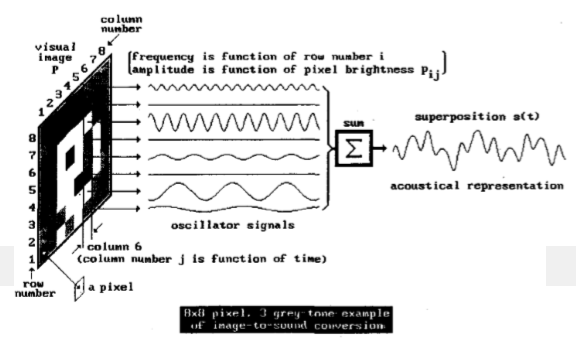
\includegraphics[width=1\textwidth]{image_to_sound}
\caption{\label{fig:image_to_sound} Principles of the image-to-sound mapping \cite{Meijer1992}}
\end{figure}
  
The experiment showed promising functionality to convert images to sound but lacks a field study test on people with blindness. Moreover, the advantages and disadvantages of this system is yet to be proven. This questions the reliability of the system since there is no recordings of tested data presented in the article of the experiment. However the sound theory represented in the article supports the system's functionality. The operations used in the system can also be applied in other settings than an aid for blind individuals, \todo{tåget argument} as these operations are mathematical expressions. They are therefore not limited to the use intended by Meijer.

\subsection{The Sound of Photographic Image}\label{sec:soundarticle}

A use of images for conversion into sound was performed and described in a paper by Atau Tanaka, who is the chair of digital media and director of culture lab at Newcastle University \cite{Tanaka2012}. The paper describes two processing methods that both convert images into sound.

The first method utilised two image series. The method used to create the sound from the image uses a temporal mapping and additive synthesis on raw grayscale images, by scanning every pixel. A bright pixel produced high notes and a dark pixel produced a low note \cite{Tanaka2012}.

The second method was used for an interactive art installation. The interactive art consisted of a wooden structure with panels covered in rice paper to display Tanaka's pre-processed images from one of the image series. The images were processed through re-synthesis processes, where the frequency bands where quantisized to whole tones and pentatonic, five notes on a scale were mapped, in which the key notes are played one at a time. The images were projected with pixel values from an inverted image of the original and each row displayed different frequency ranging from low to high frequencies. An example of this result can be seen in Figure \ref{fig:tanakaresynthesis}.  

\begin{figure}[!h]
\centering
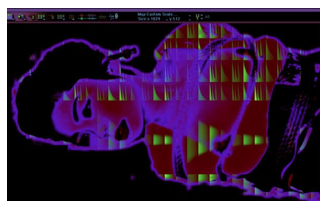
\includegraphics[width=1\textwidth]{tanakaresynthesis}
\caption{\label{fig:tanakaresynthesis}\cite{Tanaka2012}}
\end{figure}

To capture human interaction, an infrared camera on top of the installation used viewers silhouettes as a layer on the negative image which was used to reveal the original black and white image for the viewer, as seen in Figure \ref{fig:tanakainterfacepreview}.

\begin{figure}[!h]
\centering
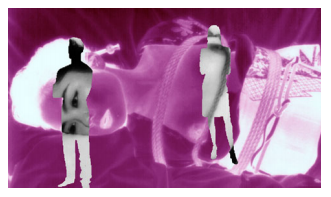
\includegraphics[width=1\textwidth]{tanakainterfacepreview}
\caption{\label{fig:tanakainterfacepreview}\cite{Tanaka2012}}
\end{figure}

This interaction also affected the produced sound which were based on the brightness of the processed image and thus produced new sounds. 

This visualisation of sound through images shows dynamic functionality of a interactive system, which utilises human interaction to alter a preprocessed image. /\todo{gå videre med praktisk anvendelse} However, since there was no evaluation of this exhibit, it is difficult to know of the practical application of these methods. This is due to it being used in an artistic way, instead of a practical one.

\section{Methods used to evaluate}\label{sec:methodsusedtoevaluate}

To produce a successful system which utilises signal inputs from an image, the theories for signal processing must be defined and discussed to gain knowledge of different varieties. This section will go through sound analysis methods and chosen filters for this project. 

\subsection{Spectrogram}\label{sub:spectrogram}

https://www.izotope.com/en/community/blog/tips-tutorials/2014/09/understanding-spectrograms/

\todo{spektrogrammer viser en fordeling af frekvenser over tid} A spectrogram is a graphical representation of sound frequencies. It can be expressed as either a two-dimensional or three-dimensional coordinate system. A two-dimensional coordinate system based on sound waves shows a change in frequency over time, hence usually having frequency on the vertical axis and time on the horizontal axis. \todo {Indsæt venligst et billede af de 2 spectrogrammer og ref}

An image has also parameters such as the \todo{synonymer} amplitude and magnitude provided through grey scaling an image. \todo{indsæt ref.} With lighter pixel values, the greater the amplitude and magnitude though it is possible to convert the colors to a third axis and and therefore produce a three-dimensional spectrogram.

By grey scaling an image and committing these values to a spectrogram, they can be further analysed in a Fourier transform.  

\subsection{Fourier transform}\label{sub:fourier}

To utilise a potential given signal by an input image, the Fourier transformation can take a given signal and \todo{den deler det op i mindre bidder på frekvens-aksen} break it down into smaller pieces. A given signal could be a time-based pattern and return the \todo{hvilken "overall cycle"? energifordeling for hver frekvens} overall cycle by applying filters, which measures individual properties upon request and returns the amount of each property and lists them. 

\begin{figure}
\caption{The mathematical expression of the Fourier transform}
\centering
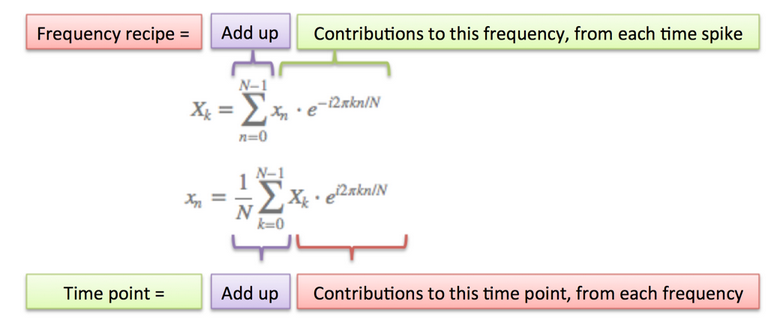
\includegraphics[width=1\textwidth]{MathFourier}
\end{figure}

The first equation process the amount of frequency k in the signal expressed as \(X_k\). The equation uses the sum of the number of time samples given \(N\) and the current sample number of time samples considered \(n\). Thus it uses the expression \(x_n\), which is the value of the signal at time \(n\), and takes \todo{in what circular path?} the backwards-moving circular path of the signal with the speed in radians times the percent of the time \(n/N\) the signal has been looked through. The circular path is the size, speed and starting angle of a given signal also defined as amplitude, frequency and phase.      

This process has the benefits of simplifying the signal by separating the important parts such as frequency, which then can be boosted and also neglect unwanted properties.       

\section{State of the art}\label{sec:stateart}
In this project, software that allows images to be converted into sounds are to be considered as the state of the art, as they are closely related to the topic of the project.

\subsection{SonicPhoto}\label{sub:sonic}
SonicPhoto \cite{White2013} is a commercial piece of software developed for windows that allows a user to input an image and converts it into unique sounds. The software interprets the image as a spectrogram, having pitch on the y-axis and time on the x-axis. The intensity of the pixels is interpreted as the amplitude of the sound. 

\begin{figure}[!h] 
\centering
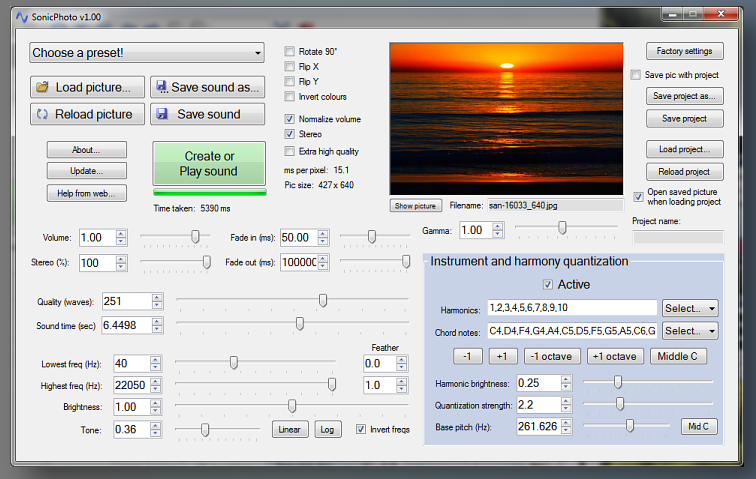
\includegraphics[width=1\textwidth]{sonicphoto}
\caption{\label{fig:sonicphoto} Interface of SonicPhoto \cite{White2013}}
\end{figure}

The software allows for customisation, such as being able to change the note harmonics, which cord nodes are played, the base of the pitch, the lowest and highest frequencies. It is also possible to edit the image; changing the alpha channel, rotation, flipping it on the x or y-axis, and inverting the colours. 

\subsection{MetaSynth}\label{sub:metasynth}
MetaSynth, a software for OSX, is also an image-to-sound conversion software. It resembles SonicPhoto by being able to import an image and edit it by for example flipping, rotating, adjusting gamma, blurring. However, MetaSynth has additional functionality for editing the output sound, as the user can add effects like  convolution, grain, delay, reverb, and chorus. The image is interpreted as a spectrogram by the software.

\begin{figure}[!h] 
\centering
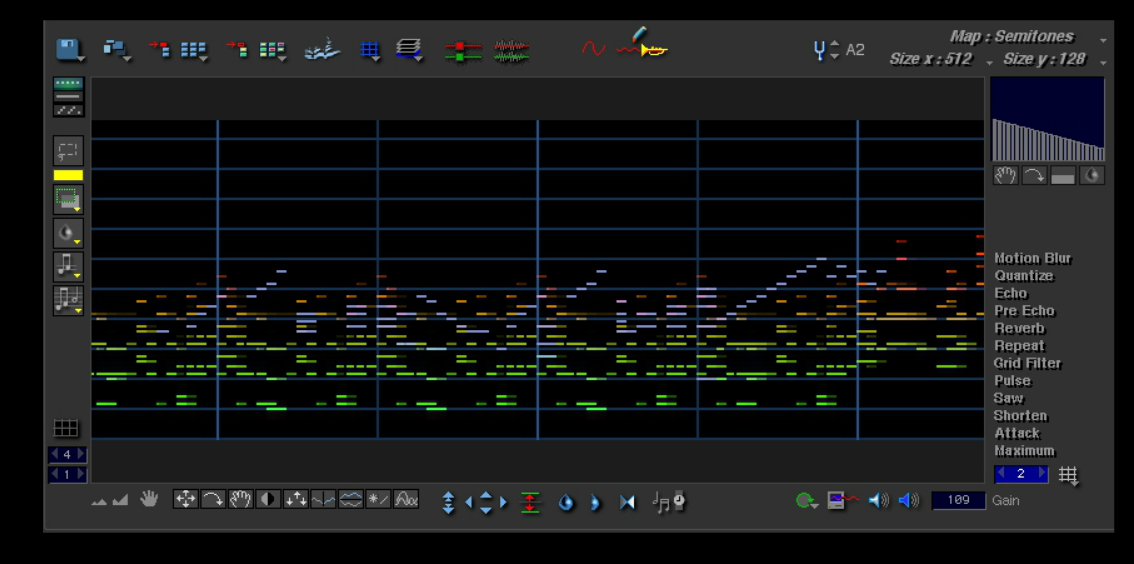
\includegraphics[width=1\textwidth]{metasynth}
\caption{\label{fig:metasynth} Interface of MetaSynth \cite{UISoftware2014}}
\end{figure}

There is also the possibility to draw freely on an image, while still having all the previously mentioned customisation for both image and sound. In this software, the color of the image determines the stereo placement. Green color for the right stereo, red for the left stereo and yellow in the center. Intensity determines the amplitude. 
Compared to SonicPhoto, MetaSynth emphasises on making music in addition to just making sounds. This is because the program allows for adding or putting the audio that the user has created into a sequence to create longer soundtracks.